%
% File naacl2019.tex
%
%% Based on the style files for ACL 2018 and NAACL 2018, which were
%% Based on the style files for ACL-2015, with some improvements
%%  taken from the NAACL-2016 style
%% Based on the style files for ACL-2014, which were, in turn,
%% based on ACL-2013, ACL-2012, ACL-2011, ACL-2010, ACL-IJCNLP-2009,
%% EACL-2009, IJCNLP-2008...
%% Based on the style files for EACL 2006 by 
%%e.agirre@ehu.es or Sergi.Balari@uab.es
%% and that of ACL 08 by Joakim Nivre and Noah Smith

\documentclass[11pt,a4paper]{article}
\usepackage[hyperref]{naaclhlt2019}
%\usepackage[nohyperref]{naaclhlt2019}

\usepackage{times}
\usepackage{latexsym}

\usepackage{url}
\usepackage{graphicx}
\usepackage{amsmath,amsfonts,amssymb}
\usepackage{paralist}
\usepackage{color,xcolor}
\usepackage{bm}
\usepackage{multirow}
\usepackage{makecell}
\usepackage{caption}
\usepackage[linesnumbered,lined]{algorithm2e}
\usepackage{todonotes}

%\aclfinalcopy % Uncomment this line for the final submission
%\def\aclpaperid{***} %  Enter the acl Paper ID here

%\setlength\titlebox{5cm}
% You can expand the titlebox if you need extra space
% to show all the authors. Please do not make the titlebox
% smaller than 5cm (the original size); we will check this
% in the camera-ready version and ask you to change it back.

% Custom commands

% bold x for equations
\newcommand{\rmx}{\mathrm x} 
% used for table headers
\newcommand{\tabh}[1]{\multicolumn{1}{c|}{\textbf{#1}}}  
\newcommand{\tabhr}[1]{\multicolumn{1}{|c||}{\textbf{#1}}}  
% used for the top left cell in a table
\newcommand{\tabc}[2]{\multicolumn{1}{|c||}{\multirow{#1}{*}{\textbf{#2}}}} 
% used for denoting the loss symbol with a subscript
\newcommand{\loss}[1]{J_{\text{#1}}}
% used for denoting the lambda symbol with a subscript
\newcommand{\hyp}[1]{\lambda_{\text{#1}}}
% used for denoting the theta symbol with a subscript
\newcommand{\nnweight}[1]{\bm{\theta_{\text{#1}}}}
% used for denoting the weight symbol (w) with a subscript
\newcommand{\weight}[1]{W_{\text{#1}}}
% used for denoting the bias symbol (b) with a subscript
\newcommand{\bias}[1]{\bm{b_{\text{#1}}}}
% custom author-year citation
% \newcommand{\citeay}[1]{\citeauthor{#1} \shortcite{#1}}

\title{Disentangled Representation Learning for\\Non-Parallel Text Style Transfer}

%\author{
%	Vineet John \\
%	University of Waterloo \\
%	{\tt vineet.john@uwaterloo.ca} \\
%	\And
%	Lili Mou \\
%	AdeptMind Research \\
%	{\tt doublepower.mou@gmail.com}\\{\tt lili@adeptmind.ai} \\
%	\AND
%	Hareesh Bahuleyan \\
%	University of Waterloo \\
%	{\tt hpallika@uwaterloo.ca} \\
%	\And
%	Olga Vechtomova \\
%	University of Waterloo \\
%	{\tt ovechtom@uwaterloo.ca} \\
%}

\date{}
\begin{document}
\maketitle
\graphicspath{{images/}}

\begin{abstract}
	This paper tackles the problem of disentangling the latent representations of style and content in language models. We propose a simple yet effective approach, which incorporates auxiliary multi-task and adversarial objectives, for style prediction and bag-of-words prediction, respectively. We show, both qualitatively and quantitatively, that the style and content are indeed disentangled in the latent space. This disentangled latent representation learning can be applied to style transfer on non-parallel corpora. We achieve high performance in terms of transfer accuracy, content preservation, and language fluency, in comparison to previous state-of-the-art approaches.\footnote{Our code is available at \url{bit.ly/2wxps69}. The materials are properly anonymized during double-blind review.}
	% \footnote{\url{https://github.com/vineetjohn/linguistic-style-transfer}}.
\end{abstract}

% 


\section{Introduction}

The neural network has been a successful learning machine during the past decade due to its highly expressive modeling capability, which is a consequence of multiple layers of non-linear transformations of input features.
Such transformations, however, make intermediate features ``latent,'' in the sense that they do not have explicit meaning and are not interpretable.
Therefore, neural networks are usually treated as black-box machinery.

Disentangling the latent space of neural networks has become an increasingly important research topic.
In the image domain, for example, \citet{chen2016infogan} use adversarial and information maximization objectives to produce interpretable latent representations that can be tweaked to adjust writing style for handwritten digits, as well as lighting and orientation for face models.
\citet{mathieu2016disentangling} utilize a convolutional autoencoder to achieve the same objective.
However, this problem is not well explored in natural language processing.

In this paper, we address the problem of disentangling the latent space of neural networks for text generation.
Our model is built on an autoencoder that encodes a sentence to the latent space (vector representation) by learning to reconstruct the sentence itself.
We would like the latent space to be disentangled with respect to different features, namely, \textit{style} and \textit{content} in our task.

To accomplish this, we propose a simple yet effective approach that combines multi-task and adversarial objectives.
We artificially divide the latent representation into two parts: the style space and content space, where we consider the sentiment of a sentence as its style.
We design auxiliary losses, enforcing the separation of style and content latent spaces.
In particular, the multi-task loss operates on a latent space to ensure that the space does contain the information we wish to encode.
The adversarial loss, on the contrary, minimizes the predictability of information that should not be contained in that space.
In previous work, researchers typically work with the style, or specifically, sentiment space~\cite{hu2017toward,shen2017style,fu2018style}, but simply ignore the content space, as it is hard to formalize what ``content'' actually refers to.

In our paper, we propose to approximate the content information by bag-of-words (BoW) features, where we focus on style-neutral, non-stopwords.
Along with traditional style-oriented auxiliary losses, our BoW multi-task loss and BoW adversarial loss enable better disentanglement of the style and content spaces.

The learned disentangled latent space can be directly used for text style transfer, which aims to transform a given sentence to a new sentence with the same content but a different style.
We follow the setting where we train our model on a non-parallel but style-labeled corpora~\cite{hu2017toward,shen2017style}, and call it \textit{non-parallel text style transfer}.
With our disentangled latent space, we simply use the autoencoder to encode the content vector of a sentence, but ignore its encoded style vector.
We then infer from the training data an empirical embedding of the style that we would like to transfer to.
The encoded content vector and the empirically-inferred style vector are concatenated and fed to the decoder.
This grafting technique enables us to obtain a new sentence similar in content to the input sentence, but with a different style.
We conducted experiments on two customer review datasets.
Qualitative and quantitative results show that both the style and content spaces are indeed disentangled well.
In the style-transfer evaluation, we achieve high performance in style-transfer accuracy, content preservation, as well as language fluency, compared with previous results.
Ablation tests also show that the auxiliary losses can be combined well, each playing its own role in disentangling the latent space.


\section{Related Work}

Disentangling neural networks' latent space has been explored in the image processing domain in recent years, and researchers have successfully disentangled features like rotation, color, etc. in images~\cite{chen2016infogan,luan2017deep}.
Some image characteristics (e.g., artistic style) can be captured well by certain statistics \cite{gatys2016image}.
In other work, researchers adopt data augmentation techniques to learn a disentangled latent space~\cite{kulkarni2015deep,champandard2016semantic}.

In NLP, the definition of ``style'' itself is vague, and as a convenient starting point, researchers often treat sentiment as a salient style attribute.
\citet{hu2017toward} propose to control the sentiment by using discriminators to reconstruct sentiment and content from generated sentences.
However, there is no evidence that the latent space would be disentangled by this reconstruction.
\citet{shen2017style} use a pair of adversarial discriminators to align the recurrent hidden decoder states of original and style-transferred sentences, for a given style.
\citet{fu2018style} propose two approaches: training style-specific embeddings, and training separate style-specific decoders. They apply an adversarial loss on the encoded space to discourage encoding style in the latent space of an autoencoding model.
\citet{zhao2018adversarially} extend the multi-decoder approach and use a Wasserstein-distance penalty to align content representations of sentences with different styles.
\citet{prabhumoye2018style} use a machine-translation preprocessing step to strip author style from documents, and then use a multi-decoder model to convert the result into a sentence with a specific style.
\citet{xu2018unpaired} propose using ``neutralization'' and ``emotionalization'' modules in a reinforcement learning framework.
\citet{li2018delete} use a hybrid retrieval and generation method that generates a desired sentence with input content and a retrieved style.

\citet{rao2018dear} treat the formality of writing as a style, and create a parallel corpus for style transfer with sequence-to-sequence models.
This is beyond the scope of our paper, as we focus on non-parallel text style transfer.

Our paper differs from previous work in that both our style space and content space are encoded from the input, and we design several auxiliary losses to ensure that each space encodes and only encodes the desired information.
Such disentanglement of latent space has its own research interest in the deep learning community.
It can also be directly applied to non-parallel text style-transfer tasks, as in the aforementioned studies.


\section{Approach}
Figure~\ref{fig:overview} shows the overall framework of our approach.
We will first present the autoencoder, serving as our base model.
Then we design the auxiliary losses for style and content disentanglement.
Finally, we introduce our approach to style-transfer text generation.


\subsection{Autoencoder} \label{ssec:seq2seq-autoencoder}

An autoencoder encodes an input to a latent vector space, from which it reconstructs the input itself.
%This serves as our primary learning objective.
%Besides, we also use the autoencoder for text generation in the style-transfer application.

Let $\rmx=(x_1, x_2, \cdots x_n)$ be an input sequence with $n$ tokens.
The encoder recurrent neural network (RNN) with gated recurrent units~\cite[GRUs,][]{cho2014learning} encodes $\rm x$ and obtains a hidden vector representation $\bm h$, which is linearly transformed from the encoder RNN's final hidden state.

\begin{figure}[!t]
	\centering
	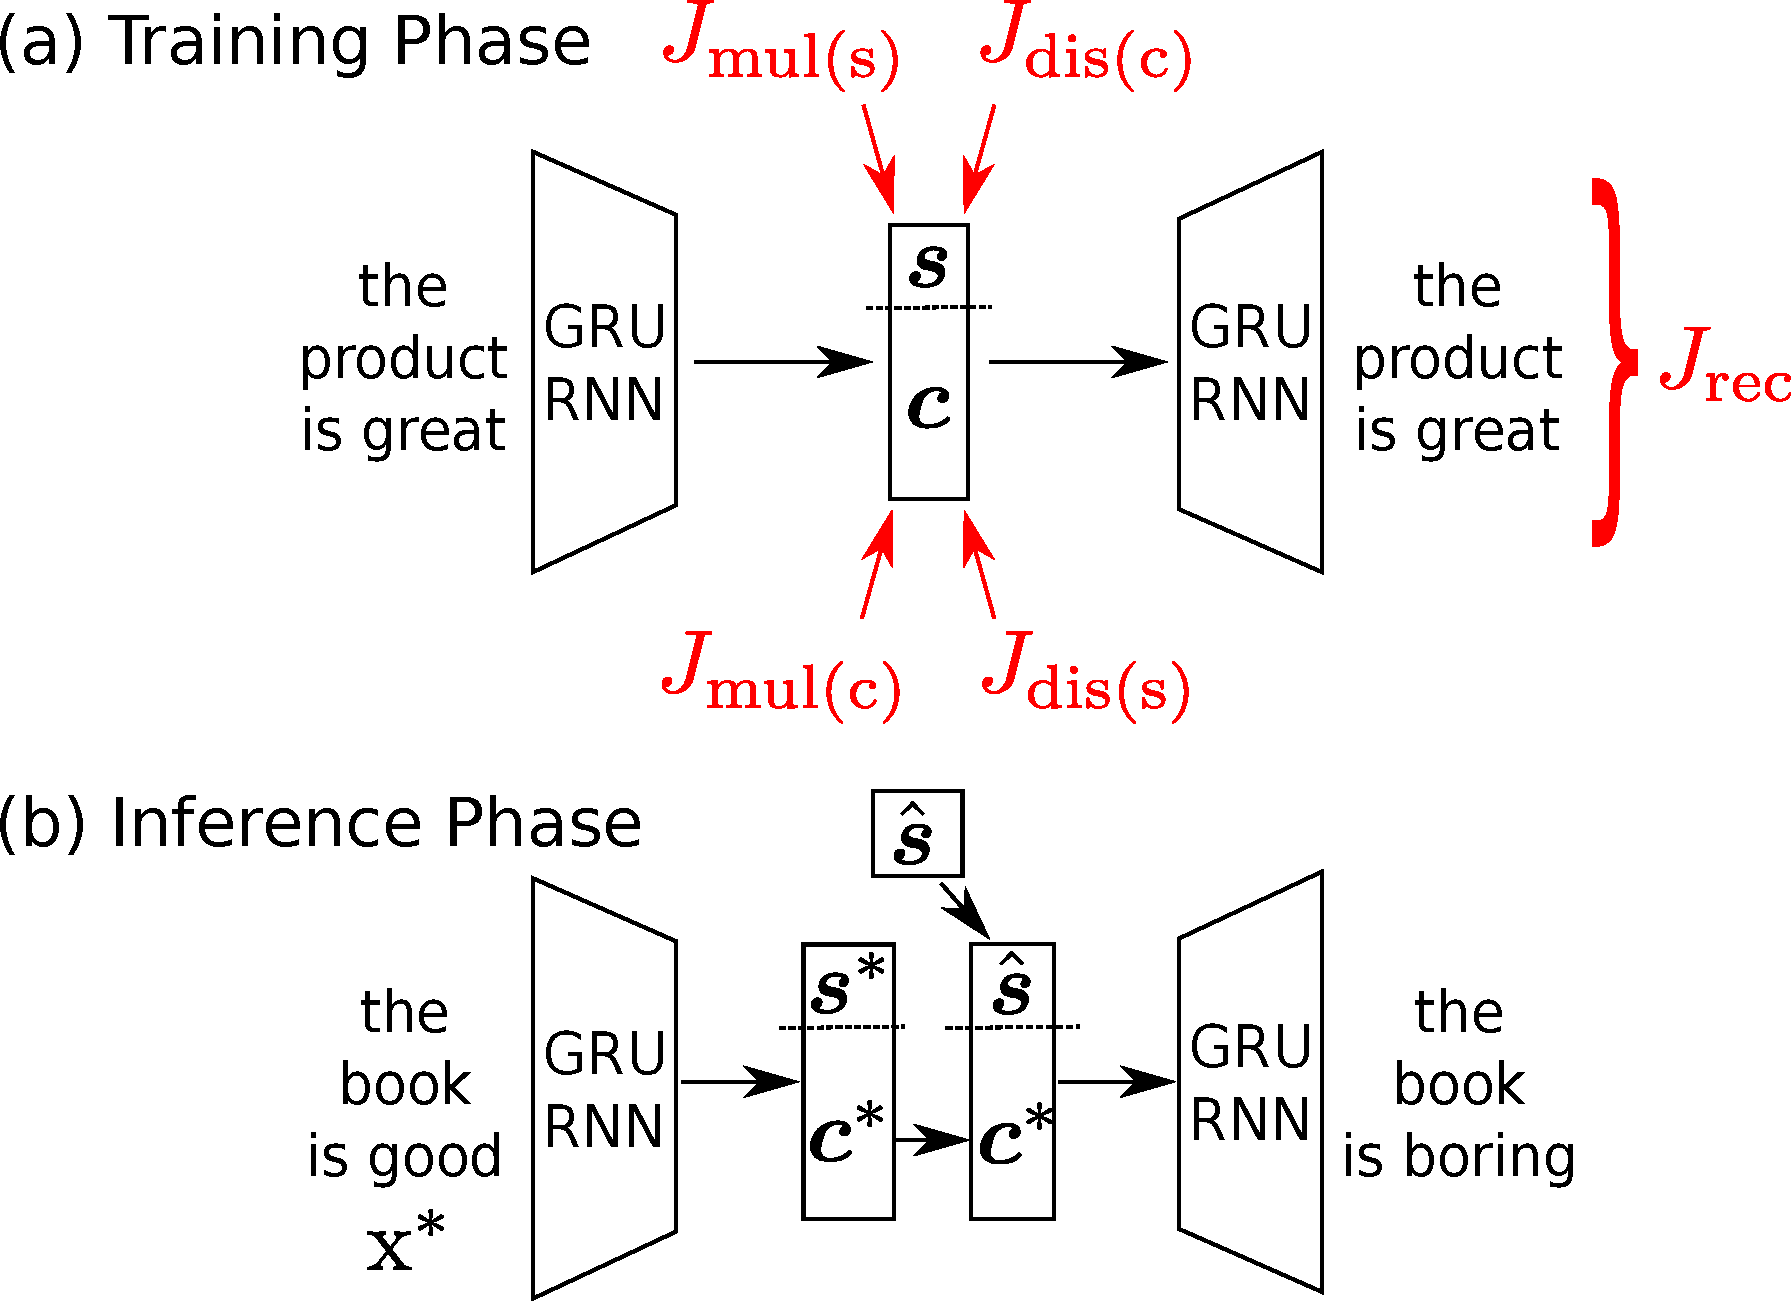
\includegraphics[width=.9\linewidth]{model-overview}
	\caption{Overview of our approach.}
	\label{fig:overview}
\end{figure}

Then a decoder RNN generates a sentence, which ideally should be $\rmx$ itself.
Suppose at a time step $t$, the decoder RNN predicts the word $x_t$ with probability $p(x_t|\bm h, x_1\cdots x_{t-1})$. Then, the autoencoder is trained with a sequence-aggregated cross-entropy loss, given by
\begin{equation}\nonumber
	\loss{AE}(\nnweight{E},\nnweight{D})= -\sum\nolimits_{t=1}^n \log p(x_t|\bm h, x_1\cdots x_{t-1})
\end{equation}
where $\nnweight{E}$ and $\nnweight{D}$ are the parameters of the encoder and decoder, respectively.
For brevity, we only present the loss for a single data point (i.e., a sentence) throughout the paper. Total loss sums over all data points, and is implemented with mini-batches.
Both the encoder and decoder are deterministic functions in the original model~\cite{rumelhart1985learning}, and thus, we call it a \textit{deterministic autoencoder} (DAE).


\textbf{Variational Autoencoder.} Alternatively, we may use a variational autoencoder~\cite[VAE,][]{kingma2013auto}, which imposes a probabilistic distribution on the latent vector. The decoder reconstructs data based on the sampled latent vector from its posterior, and the Kullback--Leibler~(KL, \citeyear{kullback1951information}) divergence  is penalized for regularization.

Formally, the autoencoding loss in the VAE is
\begin{align}
	\loss{AE}(\nnweight{E}, \nnweight{D}) = & - \mathbb{E}_{q_{E}(\bm h|\rmx)} [\log p(\rmx|\bm h)]  \nonumber \\ \nonumber
	                                        & + \hyp{kl}\operatorname{KL}(q_{E}(\bm h|\rmx)\|p(\bm h))
\end{align}
where $\hyp{kl}$ is the hyperparameter balancing the reconstruction loss and the KL term. $p(\bm h)$ is the prior, typically the standard normal  $\mathcal{N}(\bm 0,\mathrm I)$. $q_E(\bm h|\mathrm x)$ is the posterior in the form $\mathcal{N}(\bm \mu,\operatorname{diag} \bm\sigma^2)$, where $\bm\mu$ and $\bm\sigma$ are predicted by the encoder.

Compared with DAE, the reconstruction of VAE is based on the samples of the posterior, which populates encoded vectors in the neighbourhood of the prior and thus smooths the latent space.
\citet{bowman2016generating} show that VAE enables more fluent sentence generation from a latent space than DAE.

The above autoencoding losses serve as our primary training objective.
We also design several auxiliary losses to disentangle the latent space. In particular, we hope that $\bm h$ can be separated into two spaces $\bm s$ and $\bm c$, representing style and content, respectively, i.e., $\bm h = [\bm s ; \bm c]$, where $[\cdot;\cdot]$ denotes concatenation.
This is accomplished by the auxiliary losses described in the rest of this section, and shown in Figure \ref{fig:overview}a.


\subsection{Style-Oriented Losses}

We first design auxiliary losses that ensure the style information is contained in the style space~$\bm s$.
This involves a multi-task loss that ensures $\bm s$ is discriminative for the style, as well as an adversarial loss that ensures $\bm c$ is not.

\textbf{Multi-Task Loss for Style.} In the dataset, each sentence is labeled with its style (positive or negative), particularly, binary sentiment, following most previous work~\cite{hu2017toward,shen2017style,fu2018style,zhao2018adversarially}.

We build a two-way softmax classifier (equivalent to logistic regression) on the style space $\bm s$ to predict the style label, given by
\begin{equation} \label{eqn:class-pred}
	\bm y_s = \operatorname{softmax}(\weight{mul(s)} \bm s + \bias{mul(s)})
\end{equation}
where $\nnweight{mul(s)}=[\weight{mul(s)}; \bias{mul(s)}]$ are parameters for multi-task learning of style, and $\bm y_s$ is the output of softmax layer.

The classifier is trained with cross-entropy loss against the ground-truth distribution $t_s(\cdot)$ by
\begin{equation} \label{eqn:style-multi-task-loss}
	\loss{mul(s)}(\nnweight{E};\nnweight{mul(s)}) = - \sum_{l\in\text{labels}} t_s(l)\log y_s(l)
\end{equation}

In fact, we train the style classifier at the same time as the autoencoding loss.
Thus, this could be viewed as \textit{multi-task} learning, incentivizing the entire model to not only decode the sentence, but also predict its sentiment from the style vector $\bm  s$.
We denote it by ``mul(s).''
The idea of multi-task losses is not new and has been used in previous work for sentence representation learning \cite{jernite2017discourse} and sentiment analysis \cite{balikas2017multitask}, among others.


\textbf{Adversarial Loss for Style.}
The multi-task loss only ensures that the style space contains style information.
However, the content space might also contain style information, which is undesirable for disentanglement.

We thus apply an adversarial loss to discourage the content space containing style information.
We first train a classifier, called an \textit{adversary}, that deliberately discriminates the style label using the content vector $\bm c$.
Then, the encoder is trained to encode a content space from which its adversary cannot predict the style.

Concretely, the adversarial discriminator and its training objective have a similar form as Eqns.~\ref{eqn:class-pred}--~\ref{eqn:style-multi-task-loss}, but with different input and parameters, given by
\begin{align}
	\label{eqn:adv-disc-loss}
	\bm y_s                          & = \operatorname{softmax}(\weight{dis(s)} \bm c + \bias{dis(s)}) \\
	\loss{dis(s)}(\nnweight{dis(s)}) & = - \sum\nolimits_{l\in\text{labels}} t_c(l)\log y_s(l)
\end{align}
where $\nnweight{dis(s)}=[\weight{dis(s)}; \bias{dis(s)}]$ are the parameters of the adversary.

It should be emphasized that, for the adversary, the gradients are not propagated back to the autoencoder, i.e., the variables in  $\bm c$ are treated as shallow features. Therefore, we view $\loss{dis(s)}$ as a function of $\nnweight{dis(s)}$ only, whereas $\loss{mul(s)}$ is a function of both $\nnweight{E}$ and $\nnweight{mul(s)}$.

Having trained an adversary, we would like the autoencoder to be tuned in such an \textit{ad hoc} fashion that $\bm c$ is not discriminative for style.
In existing literature, there could be different approaches, for example, maximizing the adversary's loss~\cite{shen2017style,zhao2018adversarially} or penalizing the entropy of the adversary's prediction~\cite{fu2018style}.
In our work, we adopt the latter, as it can be easily extended to multi-category classification, used in Subsection~\ref{ss:content}. Formally, the adversarial objective for the style is to maximize
\begin{equation} \label{eqn:advs}
	\loss{adv(s)}(\nnweight{E})=\mathcal{H}(\bm y_s|\bm c; \nnweight{dis(s)})
\end{equation}
where $\mathcal{H}(\bm p)=-\sum_{i\in\text{labels}}p_i\log p_i$ and $\bm y_s$ is the predicted distribution over the style labels. Here, $\loss{adv(s)}$ is maximized with respect to the encoder $\nnweight{E}$ and we fix $\nnweight{dis(s)}$. The objective attains maximum value when $\bm y_s$ is uniform.

While adversarial loss has been explored in previous style-transfer papers~\cite{shen2017style,fu2018style}, it has not been combined with the multi-task loss. As shown in our experiments, combining these two losses is promisingly effective, achieving better style transfer performance than a variety of previous state-of-the-art methods.

\subsection{Content-Oriented Losses}\label{ss:content}

The above style-oriented losses only regularize style information, but they do not impose any constraint on how the content information should be encoded. In most previous work, the treatment of content is also missing~\cite{hu2017toward,shen2017style,fu2018style}.

In practice, the style space is usually smaller than content space. But it is unrealistic to expect that the content would not flow into the style space simply because of its limited capacity. Therefore, we need to design content-oriented losses to regularize the content information.

Inspired by the above combination of multi-task and adversarial losses, we apply the same idea to the content space. However, it is usually hard to define what ``content'' actually refers to.

To this end, we propose to approximate the content information by bag-of-words (BoW) features.
The BoW feature of a sentence is a vector, each element indicating the probability of a word's occurrence.
For a sentence $\rmx$ with $N$ words, the word $w_*$'s BoW probability is
$t_c(w_*)=\frac{\sum_{i=1}^{N}{\mathbb{I}\{w_i = w_*\}}}{N}$,
where $\mathbb{I\{\cdot\}}$ is an indicator function.
Here, we only consider content words, excluding stopwords and style-specific words~\cite{hu2004mining},\footnote{\url{https://www.cs.uic.edu/~liub/FBS/sentiment-analysis.html\#lexicon}} since we focus on ``content'' information.
The effect of using different vocabularies for BoW is analyzed in Supplemental Material~B.

\textbf{Multi-Task Loss for Content.} Similar to the style-oriented loss, the multi-task loss for content, denoted as ``mul(c),'' ensures that the content space $\bm c$ contains content information, i.e., BoW features.
We introduce a softmax classifier over the BoW vocabulary
\begin{equation} \label{eqn:bow-pred}
	\bm y_c = \operatorname{softmax}({\weight{mul(c)}} \bm c + \bias{mul(c)})
\end{equation}
where $\nnweight{mul(c)}\!\!=\!\![\weight{mul(c)}; \bias{mul(c)}]$ are the classifier's parameters; $\bm y_c$ is the predicted BoW distribution.

The training objective is a cross-entropy loss against the ground-truth distribution $t_c(\cdot)$, given by
\begin{equation}\label{eqn:content-multi-task-loss}
	\loss{mul(c)}(\nnweight{E};\nnweight{mul(c)}) = -\!\! \sum\nolimits_{w\in\text{vocab}}\!\! t_c(w)\log y_c(w)
\end{equation}
where the optimization is performed with both encoder parameters $\nnweight{E}$ and the multi-task classifier $\nnweight{mul(c)}$.
Notice that, although the target distribution is not one-hot  for BoW, the cross-entropy loss in Eqn.~\ref{eqn:content-multi-task-loss} has the same form as Eqn.~\ref{eqn:style-multi-task-loss}.

It is also interesting that, at first glance, the multi-task loss for content appears to be redundant to the autoencoding loss, when in fact, it is not.  The autoencoding loss only requires that the model could reconstruct the sentence based on the combined content and style spaces, but does not ensure their separation. The multi-task loss focuses on content words and is applied to the content space only.

\textbf{Adversarial Loss for Content.} To ensure that the style space does not contain content information, we design our final auxiliary loss, the BoW adversarial loss for content, denoted as ``adv(c).''

We build a content adversary, a softmax classifier on the style space predicting BoW features
\begin{align}
	\label{eqn:adv-bow-disc-loss}
	\bm y_c   = \operatorname{softmax} & ({\weight{dis(c)}}^\top \bm s + \bias{dis(c)})     \\
	\loss{dis(c)}(\nnweight{dis(c)}) = & - \sum\limits_{w\in\text{vocab}} t_c(w)\log y_c(w)
\end{align}
where $\nnweight{dis(c)}=[\weight{dis(c)}; \bias{dis(c)}]$ are the classifier's parameters for BoW prediction.

The adversarial loss for the model is to maximize the entropy of the discriminator
\begin{equation}
	\loss{adv(c)}(\nnweight{E}) = \mathcal{H}(\bm y_c | \bm s; \nnweight{dis(c)})
\end{equation}
Again, $\loss{dis(c)}$ is trained with respect to the discriminator's parameters $\nnweight{dis(c)}$, whereas $\loss{adv(c)}$ is trained with respect to $\nnweight{E}$, similar to the adversarial loss for style.

Our BoW-based, content-oriented losses are novel in the style-transfer literature.
While they do not directly work with ``style,'' they regularize the content information, so that the style and content can be better disentangled.


\subsection{Training Process}

The overall loss $\loss{ovr}$ for our model comprises several terms: the reconstruction objective, the multi-task and adversarial objectives for style and content, respectively, given by
\begin{align}
	\loss{ovr} & =  \loss{AE}(\nnweight{E}, \nnweight{D})                                                                         \\
	+          & \hyp{mul(s)} \loss{mul(s)} (\nnweight{E},\nnweight{mul(s)}) - \hyp{adv(s)} \loss{adv(s)}(\nnweight{E}) \nonumber \\
	+          & \hyp{mul(c)} \loss{mul(c)} (\nnweight{E},\nnweight{mul(c)}) - \hyp{adv(c)} \loss{adv(c)}(\nnweight{E}) \nonumber
\end{align}
where $\lambda$'s are the hyperparameters that balance the autoencoding loss and these auxiliary losses.

To put it all together, the model training involves an alternation of optimizing the adversaries by $\loss{dis(s)}$ and $\loss{dis(c)}$, and the model itself by $\loss{ovr}$, shown in Algorithm~\ref{alg:training-process}.


\begin{algorithm}[!t]
	\ForEach{mini-batch}{
		minimize $\loss{dis(s)}(\nnweight{dis(s)})$ w.r.t. $\nnweight{dis(s)}$\;
		minimize $\loss{dis(c)}(\nnweight{dis(c)})$ w.r.t. $\nnweight{dis(c)}$\;
		minimize $\loss{ovr}$ w.r.t. $\nnweight{E}, \nnweight{D}, \nnweight{mul(s)}, \nnweight{mul(c)}$\;
	}
	\caption{Training process.}\vspace{-.2cm}
	\label{alg:training-process}
\end{algorithm}


\subsection{Generating Style-Transferred Sentences} \label{ssec:sentence-generation}

A direct application of our disentangled latent space is style-transfer sentence generation, i.e., we can synthesize a sentence with generally the same meaning but a different style in the inference stage.

Let $\rmx^*$ be an input sentence with $\bm s^*$ and $\bm c^*$ being the encoded style and content vectors, respectively.
If we would like to transfer its content to a different style, we compute an empirical estimate of the target style's vector $\hat{\bm s}$ using
\begin{equation*}
	\hat{\bm s}=\frac{\sum_{i\in\text{target style}}\bm s_i}{\text{\# target style samples}}
\end{equation*}
The inferred target style $\hat{\bm s}$ is concatenated with the encoded content $\bm c^*$ for decoding style-transferred sentences, as shown in Figure~\ref{fig:overview}b.


\section{Experiments}

\subsection{Datasets}

We conducted experiments on two datasets, Yelp and Amazon reviews.
Both  comprise sentences labeled by binary sentiment (positive or negative). They are used to train latent space disentanglement as well as to evaluate sentiment transfer.

\textbf{Yelp Service Reviews.}
We used the Yelp review dataset, following previous work \cite{shen2017style,zhao2018adversarially}.\footnote{The Yelp dataset is available at \url{https://github.com/shentianxiao/language-style-transfer}}
It contains 444,101, 63,483, and 126,670 labeled reviews for train, validation, and test, respectively.
The maximum length is 15 words and the vocabulary size is $\sim$9200, as in \citet{shen2017style}.

\textbf{Amazon Product Reviews.}
We further evaluate our model with an Amazon review dataset, following some other previous papers~\cite{fu2018style}.\footnote{The Amazon dataset is available at \url{https://github.com/fuzhenxin/text_style_transfer}}
It contains 559,142, 2,000, and 2,000 labeled reviews for train, validation, and test, respectively.
The maximum length is 20 words and the vocabulary size is $\sim$58k, as in \citet{fu2018style}.


\subsection{Experimental Settings}

Our RNN has a hidden state of 256-d, linearly transformed to the style space of 8-d, and the content space of 128-d. These dimensions were chosen empirically, and we found them robust to model performance.
For the decoder, we fed the latent vector $\bm h=[\bm s, \bm c]$ to the hidden state at each step.

We used the Adam optimizer \cite{kingma2014adam} for the autoencoder and the RMSProp optimizer \cite{tieleman2012lecture} for the discriminators, following stability tricks in adversarial training  \cite{arjovsky2017wasserstein}.
Each optimizer has an initial learning rate of $10^{-3}$.
Our model is trained for 20 epochs, by which time it has mostly converged.
The word embedding layer was initialized by word2vec \cite{mikolov2013distributed} trained on respective training sets.
Both the autoencoder and the discriminators are trained once per mini-batch with $\hyp{mul(s)}\!\!=\!\!10$, $\hyp{mul(c)}\!\!=\!\!3$, $\hyp{adv(s)}\!\!=\!\!1$, and $\hyp{adv(c)} = 0.03$.
These hyperparameters were tuned by a log-scale grid search within two orders of magnitude around the default value~$1$; we chose the values yielding the best validation results.

For the VAE model, the KL penalty is weighted by $\hyp{kl(s)}$ and $\hyp{kl(c)}$ for style and content, respectively.
We set both to $0.03$, tuned by the same method of log-scale grid search. During training, we also used the $\operatorname{sigmoid}$ KL annealing schedule, following \citet{bahuleyan2017variational}.


\subsection{Exp.~ I: Disentangling Latent Space}

First, we analyze how the style (sentiment) and content of the latent space are disentangled.
We train classifiers on the different latent spaces, and report their classification accuracy in Table~\ref{tab:classification-yelp}.

We see the 128-d content vector $\bm c$ is not particularly discriminative for style.
Its accuracy is slightly better than majority guess.
However, the 8-d style vector $\bm s$, despite its low dimensionality, achieves substantially higher style classification accuracy.
When combining content and style vectors, we observe no further improvement.
These results verify the effectiveness of our disentangling approach, as the style space contains style information, whereas the content space does not.

We show t-SNE plots~\cite{maaten2008visualizing} for both DAE and VAE in Figure~\ref{fig:tsne-plots}.
As seen, sentences with different styles are noticeably separated in a clean manner in the style space (LHS), but are indistinguishable in the content space (RHS).
It is also evident that the latent space learned by VAE is considerably smoother and more continuous compared with the one learned by DAE.

We show t-SNE plots for ablation tests with different combinations of auxiliary losses in Supplemental Material C.

\begin{table}[!t]
	\centering
	\resizebox{\linewidth}{!}{
		\begin{tabular}{|l||r|r||r|r|}
			\hline
			\multirow{2}{*}{\textbf{Latent Space}} & \multicolumn{2}{c||}{\textbf{Yelp}} & \multicolumn{2}{c|}{\textbf{Amazon}}                               \\
			\cline{2-5}
			                                       & \textbf{DAE}                        & \textbf{VAE}                         & \textbf{DAE} & \textbf{VAE} \\ \hline
			None (majority guess)                  & \multicolumn{2}{c||}{0.60}          & \multicolumn{2}{c|}{0.51}                                          \\ \hline
			Content space  ($\bm c$)               & 0.66                                & 0.70                                 & 0.67         & 0.69         \\ \hline
			Style space ($\bm s$)                  & 0.97                                & 0.97                                 & 0.82         & 0.81         \\ \hline
			Complete space ($[\bm s;\bm c]$)       & 0.97                                & 0.97                                 & 0.82         & 0.81         \\ \hline
		\end{tabular}}
	\caption{Classification accuracy on latent spaces.}
	\label{tab:classification-yelp}
\end{table}
\begin{figure}[!t]
	\centering
	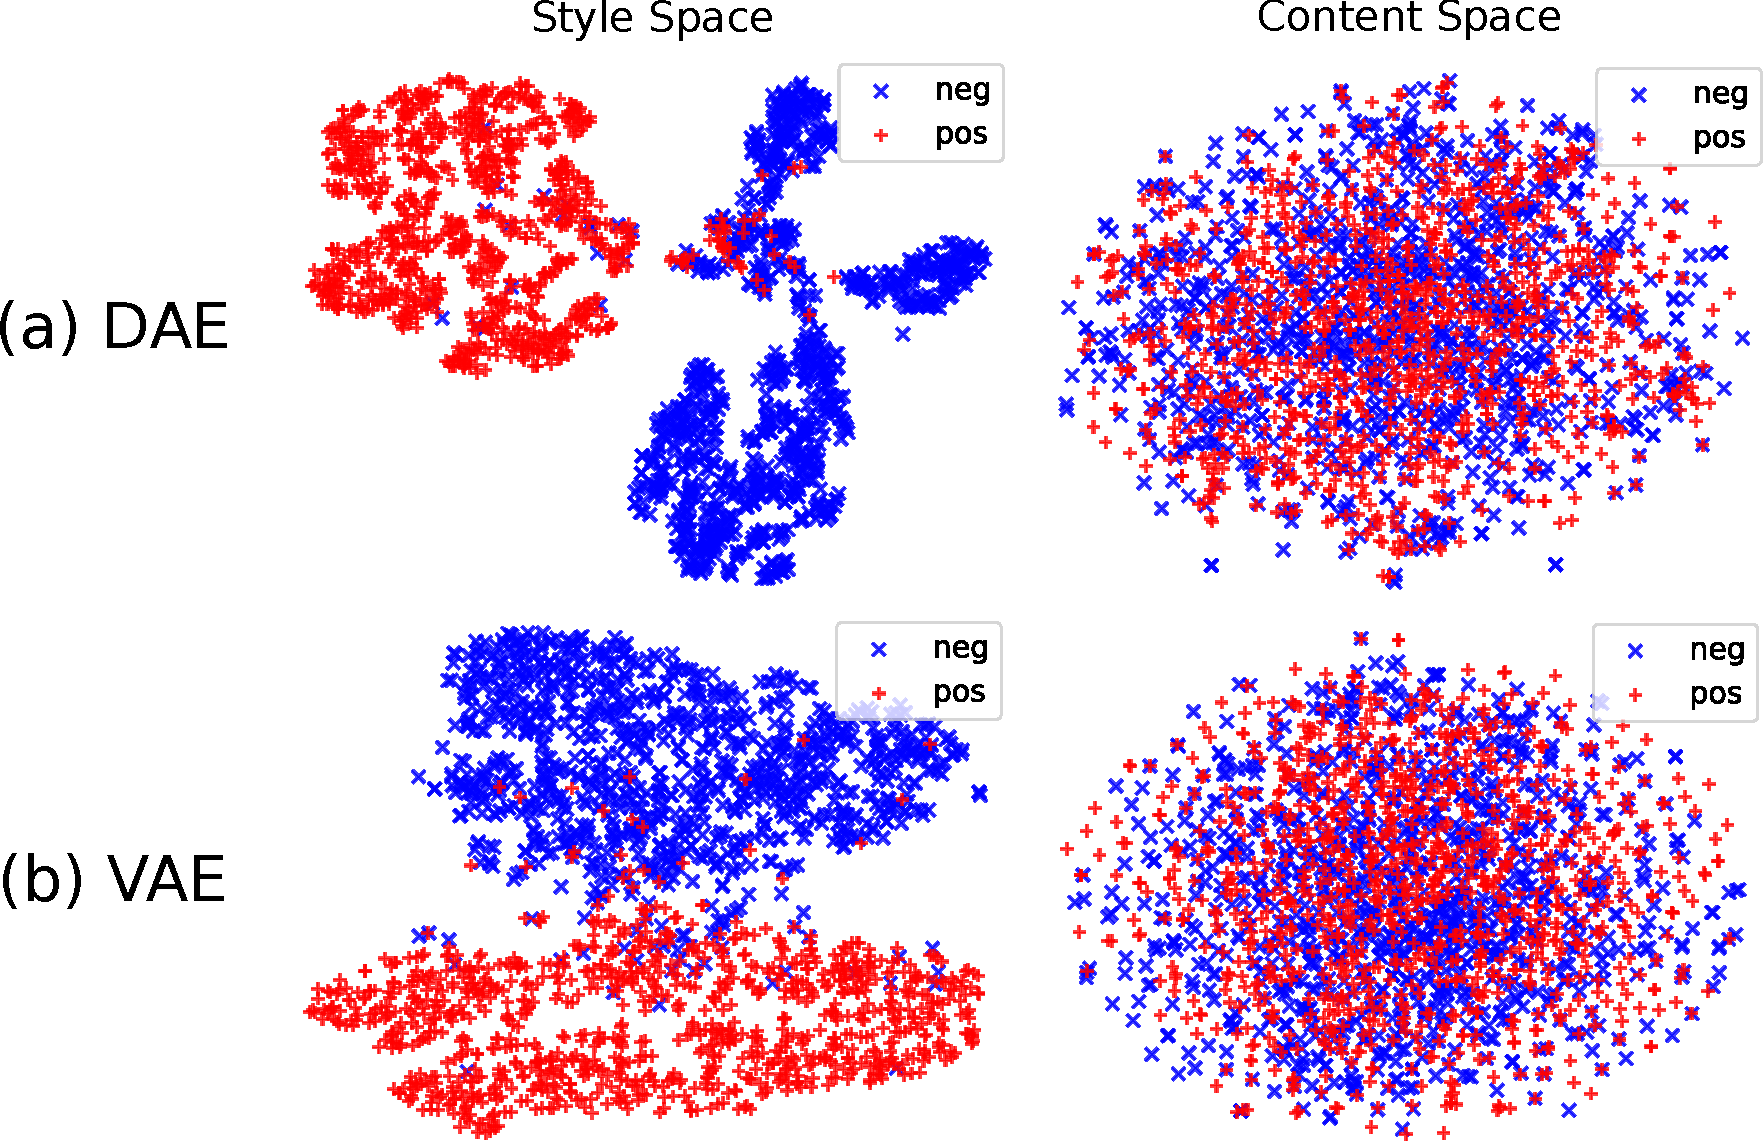
\includegraphics[width=\linewidth]{latent-spaces}
	\caption{t-SNE plots of the disentangled style and content spaces (with all auxiliary losses on the Yelp dataset).}
	\vspace{-.5cm}
	\label{fig:tsne-plots}
\end{figure}

\begin{table*}[!t]
	\centering
	\resizebox{\textwidth}{!}{
		\begin{tabular}{|l||c|c|c|c|c||c|c|c|c|c| }
			\hline
			\tabc{2}{Model}                            & \multicolumn{5}{c||}{\textbf{Yelp Dataset}} & \multicolumn{5}{c|}{\textbf{Amazon Dataset}}                                                                                                                                                                                                                           \\ \cline{2-11}
			                                           & \textbf{STA}$^\uparrow$                     & \textbf{CS}$^\uparrow$                       & \textbf{WO}$^\uparrow$ & \textbf{PPL}$^\downarrow$ & \textbf{GM}$^\uparrow$ & \textbf{STA}$^\uparrow$    & \textbf{CS}$^\uparrow$     & \textbf{WO}$^\uparrow$ & \textbf{PPL}$^\downarrow$ & \textbf{GM}$^\uparrow$     \\
			\hline\hline
			Style-Embedding \cite{fu2018style}         & \color{gray}0.18                            & \color{gray} 0.96                            & \color{gray} 0.67      & \color{gray} 124          & \color{gray} 0.10      & \color{gray} \ 0.40$^\dag$ & \color{gray} \ 0.93$^\dag$ & \color{gray} 0.36      & \color{gray} 32           & \color{gray} \textbf{0.17} \\ \hline
			Cross-Alignment \cite{shen2017style}       & \ 0.78$^\dag$                               & 0.89                                         & 0.21                   & 93                        & 0.12                   & 0.61                       & 0.89                       & 0.02                   & 202                       & 0.04                       \\ \hline
			Multi-Decoder \cite{zhao2018adversarially} & \ 0.82$^\dag$                               & 0.88                                         & 0.27                   & 85                        & 0.14                   & 0.55                       & \textbf{0.93}              & 0.17                   & 75                        & 0.11                       \\ \hline
			Del-Ret-Gen \cite{li2018delete} $^\ddag$   & 0.86                                        & \textbf{0.94}                                & 0.52                   & 70                        & 0.19                   & \color{gray}0.43           & \color{gray} 0.98          & \color{gray} 0.80      & \color{gray} 65           & \color{gray} \textbf{0.17} \\ \hline
			BackTranslate \cite{prabhumoye2018style}   & 0.85                                        & 0.83                                         & 0.08                   & 206                       & 0.07                   & \textbf{0.83}              & 0.82                       & 0.02                   & 115                       & 0.05                       \\ \hline
			Cycle-RL \cite{xu2018unpaired} $^\ddag$    & 0.80                                        & 0.92                                         & 0.43                   & 470                       & 0.09                   & 0.72                       & 0.91                       & {0.22}                 & 332                       & 0.08                       \\ \hline\hline
			Ours (DAE)                                 & 0.88                                        & 0.92                                         & \textbf{0.55}          & 52                        & 0.21                   & 0.72                       & 0.92                       & \textbf{0.35}          & 73                        & \textbf{0.15}              \\ \hline
			Ours (VAE)                                 & \textbf{0.93}                               & 0.90                                         & 0.47                   & \textbf{32}               & \textbf{0.24}          & 0.82                       & 0.90                       & 0.20                   & \textbf{63}               & 0.14                       \\ \hline
		\end{tabular}}
	\vspace{-.2cm}
	\caption{Performance of text style transfer. \textbf{STA:} Style transfer accuracy. \textbf{CS:} Cosine similarity. \textbf{WO:} Word overlap rate. \textbf{PPL:} Perplexity. \textbf{GM:} Geometric mean. The larger$^\uparrow$ (or lower$^\downarrow$), the better.  $^\dag$Quoted from previous papers (with the same data split). $^\ddag$Involving custom data splits, providing a rough (but unbiased) comparison. Others are based on our replication, and we use published code whenever possible. We achieve 0.809 and 0.835 transfer accuracy on the Yelp dataset, close to the results in \citet{shen2017style} and \citet{zhao2018adversarially}, respectively, showing that our replication is fair. Gray numbers show that a method fails to transfer style most of the time.}\vspace{-.2cm}
	\label{tab:comparison-previous}
\end{table*}


\subsection{Exp.~II: Non-Parallel Text Style Transfer}
In this experiment, we apply the disentangled latent space to sentiment-transfer text generation.

\textbf{Metrics}: We evaluate competing models based on (1) style transfer strength, (2) content preservation, and (3) quality of generated language. The evaluation of sentence generation is difficult itself in contemporary literature, so we adopt a few automatic metrics and use human judgment as well.

\textit{Style-Transfer Accuracy} (\textbf{STA}):
We follow most previous work~\cite{hu2017toward,shen2017style,fu2018style} and train a separate convolutional neural network (CNN) to predict the sentiment of a sentence~\cite{kim2014convolutional}, which is then used to approximate the style transfer accuracy.
In other words, we report the CNN classifier's accuracy on the style-transferred sentences, considering the target style to be the ground-truth.
While the style classifier itself may not be perfect, it achieves a reasonable sentiment accuracy on the validation sets ($97\%$ for Yelp; $82\%$ for Amazon).
Thus, it provides a quantitative way of evaluating the strength of style transfer.

\textit{Cosine Similarity} (\textbf{CS}):
We followed \citet{fu2018style} and computed the cosine measure between source and generated sentence embeddings, which are the concatenation of $\operatorname{min}$, $\operatorname{max}$, and $\operatorname{mean}$ of word embeddings (sentiment words removed).
This provides a rough estimation of content preservation.
%Then, we computed the cosine similarity between the source and generated sentences' embeddings, serving as a rough estimation of content preservation.

\textit{Word Overlap} (\textbf{WO}):
We find that cosine similarity, although correlated to human judgment, is not a sensitive measure.
Instead, we propose a simple, yet effective, measure that counts the unigram word overlap rate of the original sentence $\mathrm x$ and the style-transferred sentence $\mathrm y$, computed by $\frac{count(w_{\mathrm x} \cap w_{\mathrm y})}{count(w_{\mathrm x} \cup w_{\mathrm y})}$.
Here, we exclude both stopwords and sentiment words.


\textit{Perplexity} (\textbf{PPL}): We use the trigram Kneser--Ney (KN,~\citeyear{kneser1995improved}) language model as a quantitative and automated metric to evaluate the fluency of a sentence.
It estimates the empirical distribution of trigrams in a corpus, and computes the perplexity of a test sentence.
We trained the language model on the respective datasets, and report PPL on the generated sentences. A smaller PPL indicates more fluent sentences.

\textit{Geometric Mean} (\textbf{GM}):
We use the geometric mean of STA, WO, and 1/PPL---reflecting transfer strength, content preservation, and fluency, respectively---to obtain an aggregated score considering all aspects.  Notice that a smaller PPL is desired; thus, we use 1/PPL when computing GM. Also, cosine similarity (CS) is not included, because it is insensitive yet repetitive with word overlap (WO).  Here, we adopt the geometric mean so that the scale of each metric does not influence the judgment.


\textit{Manual Evaluation:}
Despite the above automatic metrics, we also conduct human evaluations to further confirm the performance of our model.
This was done on the Yelp dataset only, due to the amount of manual effort involved.
We asked 6 human annotators to rate each sentence on a 1--5 Likert scale~\cite{stent2005evaluating} in terms of transfer strength (\textbf{TS}), content preservation (\textbf{CP}), and language quality (\textbf{LQ}).
This evaluation was conducted in a strictly blind fashion: samples obtained from all evaluated models were randomly shuffled, so that the annotator was unaware of which model generated a particular sentence.
The inter-rater agreement---as measured by Krippendorff's alpha \cite{krippendorf2004content} for our Likert scale ratings---is 0.74, 0.68, and 0.72 for these three aspects, respectively. According to \citet{krippendorf2004content}, this is an acceptable inter-rater agreement. We also computed the geometric mean (\textbf{GM}) to obtain an aggregated score.

\begin{table}[!t]
	\centering
	\resizebox{.4\textwidth}{!}{
		\begin{tabular}{|l||c|c|c||c|}
			\hline
			\tabc{1}{Model}               & \textbf{TS}       & \textbf{CP}       & \textbf{CP}       & \textbf{GM}       \\
			\hline \hline
			\citet{fu2018style}           & \color{gray} 1.67 & \color{gray} 3.84 & \color{gray} 3.66 & \color{gray} 2.86 \\ \hline
			\citet{shen2017style}         & 3.63              & 3.07              & 3.08              & 3.25              \\ \hline
			\citet{zhao2018adversarially} & 3.55              & 3.09              & 3.77              & 3.46              \\ \hline \hline
			Ours (DAE)                    & 3.67              & 3.64              & 4.19              & 3.83              \\ \hline
			Ours (VAE)                    & \textbf{4.32}     & \textbf{3.73}     & \textbf{4.48}     & \textbf{4.16}     \\ \hline
		\end{tabular}}
	\caption{Manual evaluation on the Yelp dataset.}
	\vspace{-.5cm}
	\label{tab:manual-evaluation}
\end{table}



\textbf{Overall performance.}
We compare our approach with previous state-of-the-art work in Table \ref{tab:comparison-previous}.
For competing methods, we quote results from existing papers whenever possible. In some studies, the authors release their style-transferred sentences, and we tested them with our metrics. A caveat is that this may involve a different data spit, providing a rough (but unbiased) comparison. For others, we re-evaluated the model using publicly available code. We sought comparison with~\citet{hu2017toward}, but unfortunately could not find publicly available code. Instead we sought performance comparisons of their model in subsequent work, and found that, according to the human evaluation in~\citet{shen2017style}, \citet{hu2017toward} is comparable but slightly worse than \citet{shen2017style}. The latter is compared with our model in terms of both automatic metrics and human evaluation.

We can see a clear trade-off between style transfer and content preservation, as they are contradictory goals. Especially, a few models have a transfer accuracy lower than 50\%. They are shown in gray, and not the focus of the comparison, because the system cannot achieve the goal of style transfer most of the time.

Our method achieves high style-transfer accuracy (STA) in both experiments.
On Yelp, for example, VAE outperforms previous methods by more than 7\%, whereas on Amazon, VAE is 1\% lower than \citet{prabhumoye2018style}, ranking the second.

Our approach achieves high content preservation as well.
Among all the methods that can achieve more than 50\% transfer accuracy, DAE has the highest word overlap (WO) on Yelp; VAE is also high, although slightly lower than \citet{li2018delete}.
On Amazon, the phenomenon is similar. DAE is the best; VAE is 2\% lower in WO  (although 10\% better in transfer accuracy), compared with \citet{xu2018unpaired}.

For language fluency, VAE yields the best PPL in both datasets. It is also noted that, the cycle reinforcement learning (Cycle-RL) approach does not generate fluent sentences~\cite{xu2018unpaired}. They have unusually high PPL scores, but after reading the samples provided by the authors,\footnote{Via personal email correspondence.} we are assured that the sentences obtained by Cycle-RL are less fluent.

When we consider all the above aspects, our approach (either DAE or VAE) has the highest geometric meaning (GM), showing that we have achieved good performance in transfer strength, content preservation, as well as language fluency.

Table~\ref{tab:manual-evaluation} presents the results of human evaluation on selected methods.\footnote{Selection was based on the time of availability. Due to the limit of budgets, we did not re-conduct human evaluation when new approaches are published later.}
Again, we see that the style embedding model \cite{fu2018style} is ineffective as it has a very low transfer strength, and that our method outperforms other baselines in all aspects. The results are consistent with Table~\ref{tab:comparison-previous}. This implies that the automatic metrics we used are reasonable, and could be  extrapolated to different models; it also shows consistent evidence of the effectiveness of our approach.
\begin{table}[!t]
	\centering\vspace{-.2cm}\small
	\resizebox{\linewidth}{!}{
		\begin{tabular}{| l || c | c | c | c || c |}
			\hline
			\tabc{1}{Objectives}                           & \textbf{STA}                    & \textbf{CS}           & \textbf{WO}                    & \textbf{PPL}        & \textbf{GM}                    \\
			\hline\hline
			$\loss{AE}$                                    & 0.11                            & \textbf{0.94}         & \textbf{0.47}                  & 40                  & 0.11                           \\ \hline
			$\loss{AE}$, $\loss{mul(s)}$                   & 0.77                            & 0.91                  & 0.33                           & 41                  & 0.18                           \\ \hline
			$\loss{AE}$, $\loss{adv(s)}$                   & 0.78                            & 0.89                  & 0.23                           & 35                  & 0.17                           \\ \hline
			$\loss{AE}$, $\loss{mul(s)}$, $\loss{adv(s)}$  & 0.91                            & 0.87                  & 0.17                           & \textbf{23}         & 0.19                           \\ \hline
			$\loss{AE}$, $\loss{mul(s)}$, $\loss{adv(s)}$, & \multirow{2}{*}{ \textbf{0.93}} & \multirow{2}{*}{0.90} & \multirow{2}{*}{\textbf{0.47}} & \multirow{2}{*}{32} & \multirow{2}{*}{\textbf{0.24}} \\
			$\loss{mul(c)}$, $\loss{adv(c)}$               &                                 &                       &                                &                     &                                \\\hline
		\end{tabular}}\vspace{-.2cm}
	\caption{Ablation tests on  Yelp. In all variants, we follow the same protocol of style transfer by substituting an empirical estimate of the target style vector.}
	\label{tab:ablation-results}
\end{table}

\textbf{Ablation Test.} We conducted ablation tests on the Yelp dataset, and show results in Table~\ref{tab:ablation-results}. With $\loss{AE}$ only, we cannot achieve reasonable style transfer accuracy by substituting an empirically estimated style vector of the target style.  This is because the style and content spaces would not be disentangled spontaneously with the autoencoding loss alone.
With either $\loss{mul(s)}$ or $\loss{adv(s)}$, the model achieves reasonable transfer accuracy and cosine similarity. Combining them together improves the transfer accuracy to 90\%, outperforming previous methods by a margin of $5\%$ (Table~\ref{tab:comparison-previous}). This shows that the multi-task loss and the adversarial loss work in different ways. Our insight of combining the two auxiliary losses is a simple yet effective way of disentangling latent space.
However, $\loss{mul(s)}$ and $\loss{adv(s)}$ only regularize the style information, leading to gradual drop of content preserving scores. Then, we have another insight of introducing content-oriented auxiliary losses, $\loss{mul(c)}$ and $\loss{adv(c)}$ based on BoW features, which regularize the content information in the same way as style. By incorporating all these auxiliary losses, we achieve high transfer accuracy, high content preservation, as well as high language fluency.

\section{Conclusion}
In this paper, we propose an effective approach for disentangling style and content latent spaces.
We combine multi-task and adversarial objectives to separate content and style information from each other, and propose to approximate content information with bag-of-words features of style-neutral, non-stopword vocabulary.

Both qualitative and quantitative experiments show that the latent space is indeed separated into style and content parts.
The disentangled space can be directly applied to text style-transfer tasks.
It achieves high style-transfer strength, high content-preservation scores, as well as high language fluency, compared with previous work.

\bibliography{naaclhlt2019}
\bibliographystyle{acl_natbib}

\end{document}
